\chapter{Schedule}
The main tasks involving this project are:
\begin{itemize}
	\item Delivering the Requirement Analysis and Specification Document, containing the goals, the domain assumptions, and the functional and non-functional requirements of the software system.
	\item Delivering the Design Document, containing the architecture and the design of the software system.
	\item Delivering the Integration Testing Plan Document, containing the strategy used to perform integration testing on the system.
	\item Delivering the Project Plan, which is this document.
	\item Preparing a brief presentation about the delivered documents, with slides.
	\item Implementing the software system and write unit tests.
	\item Performing integration testing on the system.
\end{itemize}

Please note that, as new requirements can emerge, new choices are made and the development goes on, the process can be iterated multiple times. In particular, unit and integration testing will be continuously performed throughout the development process.

However, some tasks need to be concluded before some other can begin: the dependency graph for the activities is shown in figure~\ref{fig:dag_tasks}.

The first five tasks for the project are already defined by the document about describing the assignment, together with the deadlines for the delivery of the RASD, the Design Document and the ITPD. The date for the presentation is also fixed. So, those activities are already scheduled.

\begin{figure}[H]
	\centering
	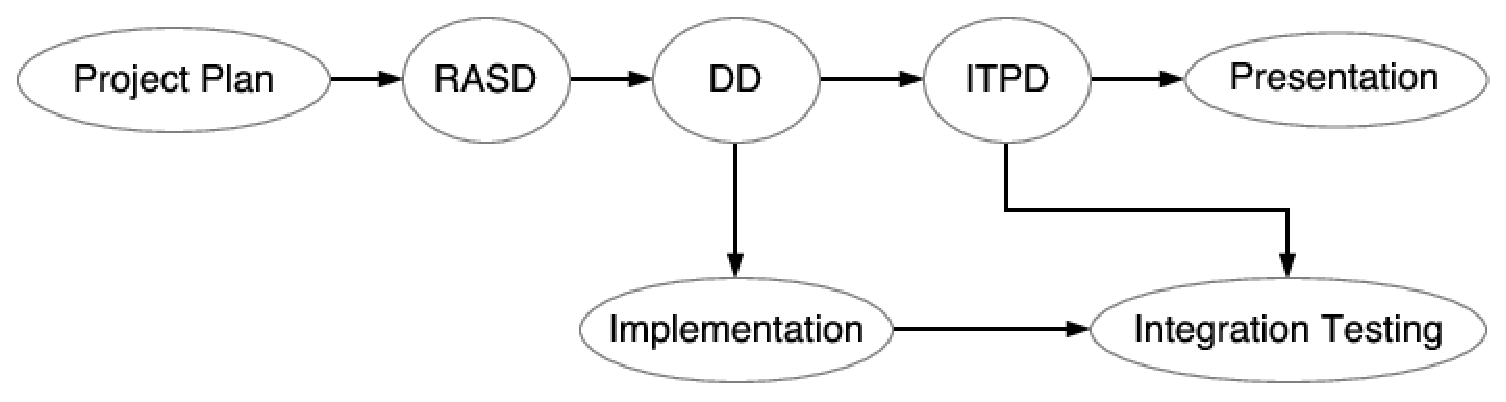
\includegraphics[width=\linewidth,keepaspectratio]{figures/dag_tasks.eps}
	\caption{DAG for the dependencies among tasks}
	\label{fig:dag_tasks}
\end{figure}

There are no fixed deadlines, instead, for the development of the software. Based on the COCOMO estimation performed in chapter 2, we expect the entire project to last 8 months, so it will be presumably finished by June 2017. The schedule for our project is outlined in table~\ref{tab:schedule}, while figure~\ref{fig:gantt} shows the Gantt chart for PowerEnJoy.

\begin{table}[H]
	\centering
	\begin{tabular}{|l|r|r|}
		\hline
		\textbf{Activity} & \textbf{Start date} & \textbf{Deadline} \\
		\hline
		RASD & 16/10/2016 & 13/11/2016 \\
		DD & 14/11/2016 & 11/12/2016 \\
		IPTD & 12/12/2016 & 15/01/2017 \\
		Project Plan & 05/01/2017 & 22/01/2017 \\
		Presentation &  &  \\
		Implementation &   &  \\
		Integration testing &   &  \\
		\hline	
	\end{tabular}

	\caption{Schedule for the project tasks}
	\label{tab:schedule}
\end{table}

\begin{figure}[H]
	\centering
	\begin{sideways}	
		\begin{ganttchart}[
			vgrid={*{6}{draw=none},dotted},
			time slot format=isodate,
			x unit=0.7mm,
			today=2017-01-22,
			today rule/.style= {ultra thick},
			today label=Today,
			link bulge=6, link tolerance=5,
			bar inline label node/.style={font=\scriptsize},
			inline
			]{2016-10-01}{2017-06-30}
			\gantttitlecalendar{year,month=name} \\
			\ganttbar[name=rasd]{RASD}{2016-10-16}{2016-11-13} \\
			\ganttbar[name=dd]{DD}{2016-11-14}{2016-12-11} \\
			\ganttbar[name=itpd]{ITPD}{2016-12-12}{2017-01-15} \\
			\ganttbar[name=pp]{PP}{2017-01-05}{2017-01-22} \\
			\ganttbar[name=pres]{Presentation}{2017-01-24}{2017-02-18} \\
			\ganttbar[name=impl]{Implementation}{2017-02-19}{2017-06-01} \\
			\ganttbar[name=int-test]{Int. Test.}{2017-06-01}{2017-06-20}
			\ganttlink{rasd}{dd}
			\ganttlink{dd}{itpd}
			\ganttlink{impl}{int-test}
		\end{ganttchart}
	\end{sideways}

	\caption{Gantt chart of the project}
	\label{fig:gantt}
\end{figure}